\begin{tikzpicture}
\draw[black] (0,0) circle (0.001cm);
\filldraw[draw = black, fill = white] (5,0) rectangle (7,2);
\draw[->] (6,0) -- (6,-2);
\draw[black] (5.75,1) node[anchor = west] {M};
\draw[black] (5.75,-2.25) node[anchor = west] {$\vec{F_1}$};
\draw[->] (7,1) -- (9,1);
\draw[black] (9,1) node[anchor = west] {$\vec{F_2}$};
\draw[->] (5,1) -- (3,1);
\draw[black] (2.5,1) node[anchor = west] {$\vec{F_3}$};
\end{tikzpicture}

Before we even begin discussing Newton’s Laws, I think it is important to talk a little bit about what it also means for something to be a force. The classic description of a force is "a push or a pull." But quite frankly I, and I don't think anyone else has any idea what this means. For example, the electromagnetic force exists, but electrons don’t “push” or “pull” on each other. Instead, they impart forces on each other. We are not going to get a rigorous definition of a force quite yet, but for now, we can classify the forces into different types. The first type of force is a contact force. These are forces in which two bodies are in contact with each other and impart an equal but opposite force on each other. You can picture this being the force between two blocks that are next to each other and touching each other. When a block is touching another block, they can impart a force on each other. The force of our hands pushing a box is an example of a contact force. 

The other type of force that we will encounter is, with little surprise, the non-contact force. An example of this type of force is the gravitational force. For now, we can think of this as being the downward pull that we experience due to to the large mass of Earth. We can also define the tension force. The clearest example of this would be the force of the string in a system with a mass connected to the bottom of the string and moving like a pendulum. The last two forces we can talk about are the magnetic and electric forces. These forces do not require anything to touch each other, and we will find out exactly how they work much later. What is important to now know is just that, even though we do not experience them nearly as much as the gravitational force, they are still present. And they are essential in many current pieces of technology. It is also important now to understand that all forces arise at the molecular level. There are uncountable numbers of particles imparting forces on each other at given times. These interactions ultimately work out to the classical world that we have. In many ways, this is really odd and extremely interesting. It is not amazing that quantum particles behave as they do, rather that everyday items behave as they do. We can think of the force of gravity on a mass due to Earth as being the sum of the forces caused by each little earth particle pulling on the mass. Each individual force is tiny, but when you sum all of the forces from the entire planet, the force will increase many orders in magnitude. We will do worked examples with this idea in lessons on gravitation. 
\newline
\newline
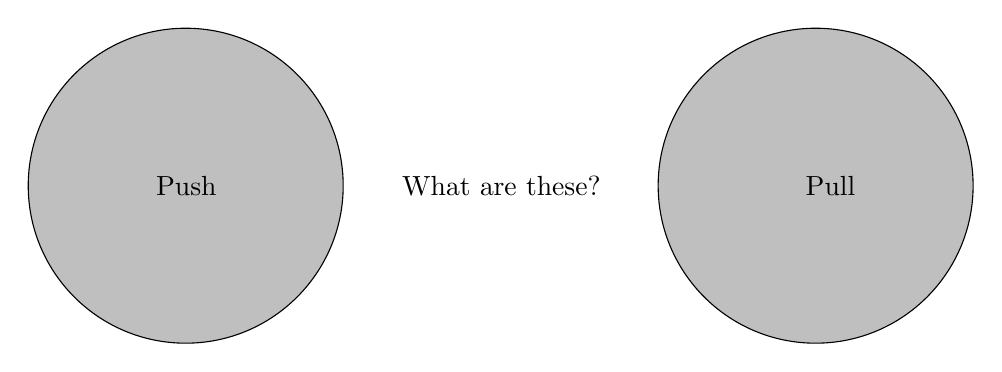
\begin{tikzpicture}
\filldraw[fill = lightgray, draw = black] (4,0) circle (2cm);
\filldraw[fill = lightgray, draw = black] (12,0) circle (2cm);
\draw[black] (3.5,0) node[anchor=west] {Push};
\draw[black] (11.75,0) node[anchor=west] {Pull};
\draw[black] (6.625,0) node[anchor=west] {What are these?};
\end{tikzpicture}
\newpage